% $Id: $
\documentclass[a4paper,12pt]{article}

\usepackage{enumerate}
\usepackage{amsmath,amsthm,amssymb}
\usepackage{amsfonts}
% The following makes latex use nicer postscript fonts.
\usepackage{times}
\usepackage{pgf,tikz}
\usepackage{hyperref}

\usetikzlibrary{arrows}
\pagestyle{empty}
\usepackage{subcaption}
\usepackage[english]{babel}
\usepackage{tikz}
%\usepackage[colorlinks,urlcolor=blue,linkcolor=blue]{hyperref}
\pagestyle{headings}
\newcommand{\upuparrow}{\mathrel{\reflectbox{\rotatebox[origin=c]{90}{$\twoheadrightarrow$}}}}
\newcommand{\downdownarrow}{\mathrel{\reflectbox{\rotatebox[origin=c]{90}{$\twoheadleftarrow$}}}}
\usepackage{vubtitlepage}
\usepackage{lmodern}
\usepackage{graphicx}

\usepackage[geometry]{ifsym}
%\usepackage[font=small,format=plain,labelfont=bf,up,textfont=it,up]{caption}
\renewcommand{\thefigure}{\thesection.\arabic{figure}}
\author{Filip Moons}
\title{Rate-monotonic scheduling}

\newtheorem{theorem}{Theorem}[section]
\newtheorem{lemma}[theorem]{Lemma}
\newtheorem{proposition}[theorem]{Proposition}
\newtheorem{conjecture}{Conjecture}

\newtheorem{property}[theorem]{Property}
\newtheorem{definition}[theorem]{Definition}
\newtheorem{method}[theorem]{Method}
\newtheorem{corollary}[theorem]{Corollary}
\newtheorem{remark}[theorem]{Remark}
\newtheorem{remarks}[theorem]{Remarks}
\newtheorem{notation}[theorem]{Notation}
\theoremstyle{definition}
\newtheorem{example}[theorem]{Example}
\newtheorem{examples}[theorem]{Examples}

\setcounter{tocdepth}{5}
\newcommand{\N}{{\mathbb N}}
\newcommand{\Z}{{\mathbb Z}}
\newcommand{\Q}{{\mathbb Q}}
\newcommand{\R}{{\mathbb R}}
\newcommand{\C}{{\mathbb C}}
\newcommand{\HQ}{{\mathbb H}}
\renewcommand{\P}{{\mathbb P}}
\newcommand{\E}{{\mathbb E}}
\newcommand{\cost}{\text{cost}}
\newcommand{\Nash}{\text{Nash}}
\newcommand{\Tau}{\mathcal{T}}
\newcommand{\nash}{\text{nash}}
\newcommand{\opt}{\text{opt}}
\newcommand{\LFP}{\text{LFP}}
\renewcommand{\int}{\text{int}}

%\newenvironment{proof}{\noindent{\bf Bewijs.}}{{\hfill $ \ Box $}\vskip 4mm}

%\promotortitle{Promotor/Promotors}
\promotor{Prof. Dr. M. Timmerman}
\advisors{}
\advisortitle{}
\addto\captionsenglish{\renewcommand*\abstractname{Abstract for non-mathematicians}}
\date{MEI 2006}
\faculty{Faculty of Science}
\advisortitle{}
\department{Department of Computer Science}
\reason{Operating systems \& security}

\date{January 2014}


\begin{document}
% Then english TitlePage
\maketitlepage


\tableofcontents
\newpage
% \pagenumbering{arabic}
\section{Introduction}
This paper gives a good overview of the basic concepts of Rate Monotonic scheduling. We first introduce
real-time operating systems, because that's the field where RMS is applied. Second, we introduce the needed definitions to know before studying the algorithm.
We make make a lot of assumptions about the tasks that must be executed, to 
become an easy configuration in which we can introduce RMS.
Next, the algorithm is introduced. The second section closes with the schedulability tests used to decide if a task set can be scheduled by RMS or not.
The next section is about extensions of the Rate Monotonic theory. It gives some examples of the theory applied on task sets with different assumptions than in section 1.
These extensions are in fact generalizations of the theory because they often just abandon some of the assumptions. We close this paper with some concrete simulations of RMS in the program Cheddar. \newpage
\section{Real-time operating systems}
A real-time operating system (RTOS) is an operating systems that serves 
real-time application request. The operating system can process data as it comes 
in, normally without notable delay. Processing times are measured in 
milliseconds. A real-time operating system has an advanced algorithm for 
scheduling it's tasks. This paper is about such an advanced algorithm: 
rate-monotonic scheduling. The real-time operating systems using RMS are the 
oftene preemptive and have quite constant response times.  Preemptive operating systems are capable of temporarily interrupting a task to give the priority to another task, without requiring cooperation of the task. The interrupted task is resumed at a later time.
\newpage
\section{Scheduling}
\subsection{Definitions}

\begin{definition}
  A \emph{task} $\tau_i$ is a process or a thread that has to be periodically 
  executed in a \emph{period} $T_i$. The worst case \emph{execution time} of a task $\tau_i$ is denoted as 
  $C_i$, with $C_i \leq T_i$. The \emph{deadline} $D_i$ of $\tau_i$ is the available time on the processor 
  the execute the task. In this paper however, we consider $D_i = T_i$. The \emph{priority}  
  of a task is indicated by it's index number: $\tau_i$ has an higher priority. 
  than $\tau_j$ when $i < j$. 
\end{definition}
\begin{definition}
  A \emph{job} of task $\tau_i$ is a single period of task $\tau_i$.
  \end{definition}
  
  \begin{definition}
  A task $\tau_i$ has a phasing $I_i$ ($0 < I_i < T_i$). This phasing 
gives the time at which the first job of $\tau_i$ occurs.
  \end{definition}

\begin{definition}
  A \textit{task set} is a set of tasks, the indexes of the task indicate the priorities of these tasks relative to each 
  other:
  $$\Tau = \{\tau_1, \tau_2, ... \tau_n\}$$
  
  \end{definition}


\begin{remark}
  In this section, we have to make some assumptions about tasks: switching between 
  tasks is instantaneous, there is no interaction between tasks, jobs are ready 
  to be executed at the beginning of their period and they quit the CPU after the job is finished. A task can only have one job that's being executed, new jobs have to wait after this job is done. 
  We also assume that a task's execution time $C_i$ is always constant.
  
  It's immediately clear that some of these assumptions 
  are not realistic in an actual real-time system. We'll study later on some extensions that can handle deviations of these assumptions. 
\end{remark}\label{assumptions}

\subsection{Sheduling algorithms}
\subsubsection{Static priority scheduling algorithms}
Static priority scheduling algorithms are algorithms in which each task is 
assigned a constant priority. The priorities are normally set before executing 
the a static priority scheduling-algorithm. 
\subsubsection{Dynamic priority scheduling algorithms}
Dynamic priority scheduling algorithms are algorithms in which each task has a 
priority that may change during the execution of a task set on the CPU. 
\subsubsection{Preemptive priority scheduling algorithms}
A preemptive priority scheduling algorithm is characterized by the fact that 
these type of algorithms may interrupt the execution of a task to prioritize the 
execution of another task on the CPU. The task that had been interrupted may resume afterwards.  

\subsubsection{Rate-monotonic scheduling}
A rate-monotonic scheduling algorithm is based on two rules
\begin{enumerate}
  \item The task with the smallest period has the highest priority,
  \item A higher-priority task ready to be executed, overrides the current 
  executed task. The current executed task is is interrupted and may resume 
  afterwards.
\end{enumerate}
From the first rule, we can conclude that RMS is a static priority scheduling 
algorithm because the priorities are assigned to the task before the task set is 
executed. The second rule implies that RMS is a preemptive priority scheduling 
algorithm because RMS stops immediately a task with lower priority (higher period) when a task 
with higher priority (lower period) is ready to be executed, so RMS is a \emph{static-priority scheduling 
algorithm}.
\subsection{Schedulability tests}
Given the execution time $C_i$, the period $T_i$ of a task $\tau_i$, the 
utilization of the CPU can be calculated as:
$$U_i = \frac{C_I}{T_i}.$$
The utilization factor of a task set $\Tau$ is defined as:
\begin{eqnarray}
  U = \sum\limits_{i=1}^{n} \frac{C_i}{T_i}
\end{eqnarray}
When  $U> 1$, it's immediately clear that the task set $\Tau$ cannot be 
executed by any scheduling algorithm (considering we only have 1 CPU).
\subsubsection{Liu \& Layland lower bound}\begin{theorem}\textbf{Schedulability test 1 for RMS}
  Liu & Layland (1973) showed that for $n$-tasks with distinct periods, a 
  feasible schedule will always exist if the utilization factor of the task set 
  is below $n(2^{\frac{1}{n}} -1)$:
  \begin{eqnarray}
  U \leq n(n(2^{\frac{1}{n}} -1)
  \end{eqnarray}
\end{theorem}\label{bound}

\begin{figure}
  \centering
  % Requires \usepackage{graphicx}
  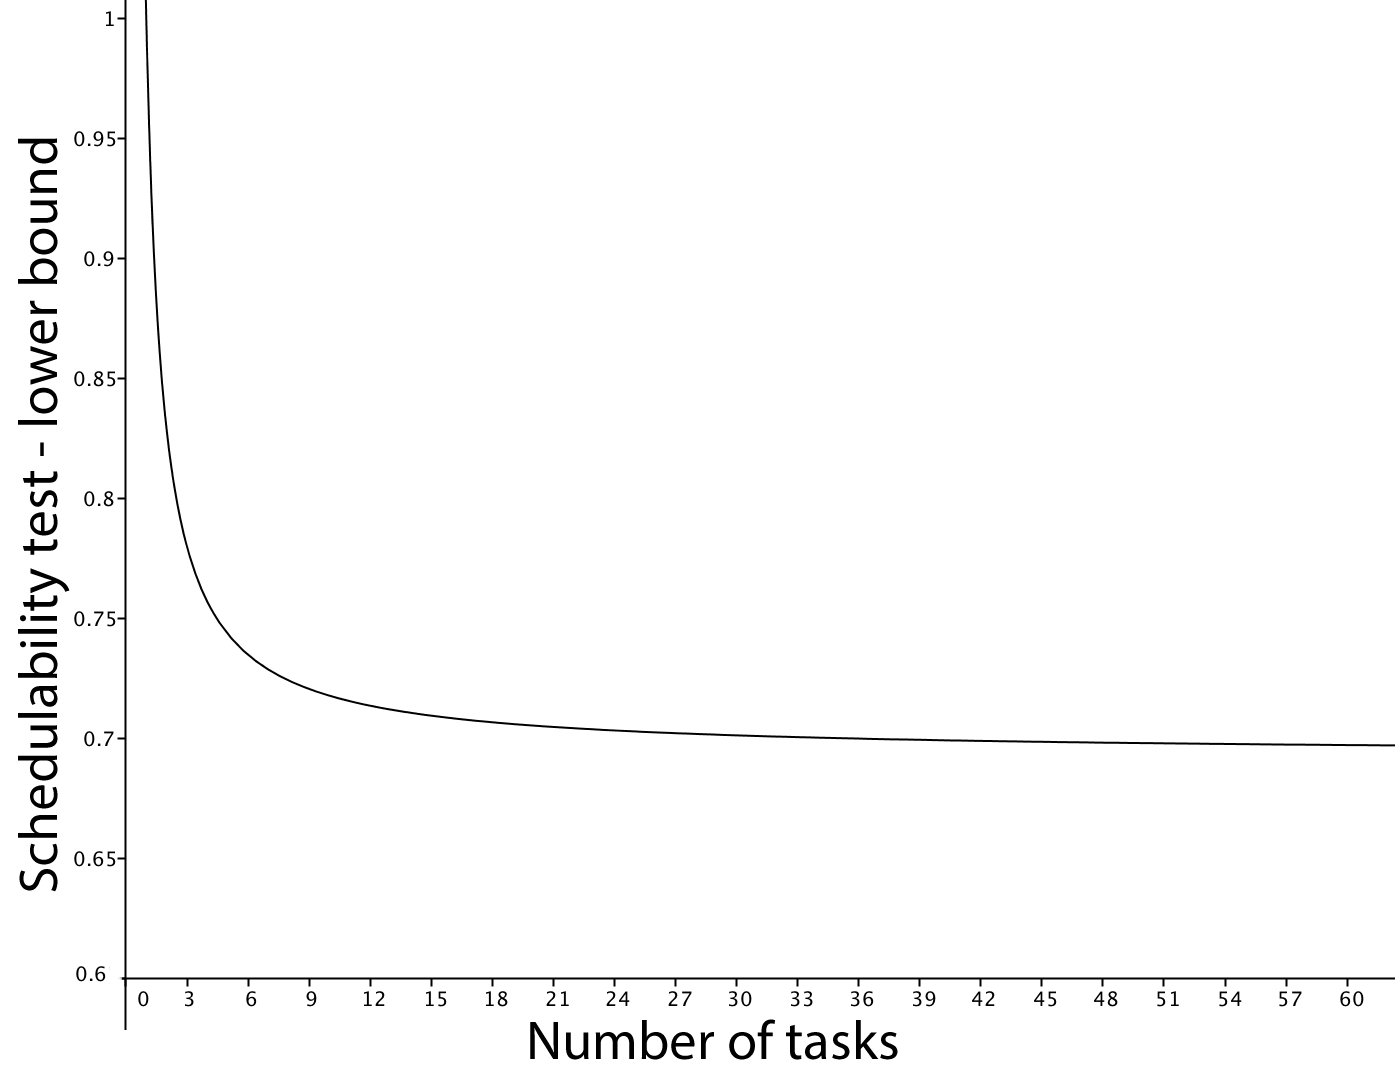
\includegraphics[scale=0.2]{grafkak.png}\\
  \caption{The louwer bound of the schedulability test}\label{scottplane}
\end{figure}
Using this theorem, we can easily find that
\begin{eqnarray}
\lim_{n \rightarrow \infty}   n(2^{\frac{1}{n}} -1) = \ln 2 \approx 
0.693147...
\end{eqnarray}\label{limiet}
Thus 0.693147... is a worst case bound for RMS. However, this approximation is only a good
approximation when the number of tasks is high enough ($> 20$ tasks).
If equation 2 is satisfied, all 
of the task will meet their deadlines.
\begin{figure}

\end{figure}
\begin{example}
  Consider these 3 tasks:
  \begin{enumerate}
    \item $\tau_1$: $T_1$ = 40 ms,  $C_1$ = 5 ms,
    \item $\tau_2$: $T_2$ = 40 ms,  $C_2$ = 7 ms,
    \item  $\tau_3$: $T_3$ = 5 ms,   $C_1$ = 2 ms,
  \end{enumerate}
  Then: $U_1 = 0.125$, $U_2 = 0.175$, $U_3 = 0.4$. With $n=3$, the sum of $U_1, U_2, U_3$ must be lower than 0.7798, using equation 2.  We become that $0.125 + 0.175 + 0.4 = 0, 575$ 
  is indeed under the limit of 0.7798. By the schedulability test, we conclude 
  that these tasks are schedulable. 
\end{example}
\subsubsection{Response time (RT) test}
Although the schedulability test may be useful, if the utilization function is 
between the worst case bound and $1$, the schedulability test for RMS is 
inconclusive. A more precise test must be used. This will be \emph{the response time (RT) 
test}. This test is based on ``worst-case phasing''. A worst-case phasing 
corresponds to a set of values for $I_i$ ($ i \in [1...n]$, with a task set of $n$ 
tasks) leading to the worst schedulable setting of $\Tau$. We now have the 
following nice theorem:
\begin{theorem}\textbf{(Response time (RT) test)}
  For a task set, 
  if each task meets its deadline with worst case task phasing, the deadline will always be 
  met.
\end{theorem}
  When does this worst case task phasing occur? Intuitively, it's clear that the 
  worst case occurs when all the task $\tau_i$ have their phasing equal to 0, so 
  $I_i=0$. This is the case when all tasks are launched at the same time. This 
  is obvious: take a random task $\tau_j$. In this scenario, the end time $= I_j + T_j = 0 + T_j = T_j$.
  Now, letting $\tau_j$ start at a different moment than the other task, is equal to changing the period of task $\tau_j$ to 
  $I_j' > 0$ extends the end time immediately.
  
  \begin{theorem}
    The worst-case phasing occurs when $I_i = 0, \forall i \in [1 .. n]$. This 
    configuration where all tasks start at the same time is often called a
    \emph{critical instance}.
  \end{theorem}
  
 Now,  remember the assumption that a task can only have one job that's being executed, new jobs have to wait after this job is done. 
This immediately leads to the following theorem, a reformulation of the RT test:

\begin{theorem}\textbf{(Reformulation - Response time (RT) test)}\label{refor}
A task set can be scheduled by RMS if the deadline of the first job of each task is met when using the scheduling algorithm starting from a critical 
instant.
\end{theorem}

\begin{remark}
  Theorem \ref{refor} applies in a much more general setting too: a periodic 
  task set can be scheduled in any static scheduling algorithm if the deadline 
of each task is met when using the scheduling algorithm starting from a critical instant. 
\end{remark}
\subsection{Time-Demand function}
Based on the above test, we conclude that the RT test requires the computation 
of the total processing time of each task in a task set. If each total processing time is 
less than it's corresponding period, the task set is schedulable. 

The total processing requirement $u_i(t)$ of a task $\tau_i$ in the time interval $[0,t]$ 
is given by, with $0<t\leq T_i$ (note that task are ordered by increasing priorities!):
\begin{eqnarray}
 u_i(t) = C_i + \sum\limits_{k=1}^{i-1} \left \lceil{\frac{t}{T_i}}\right \rceil C_k
 \end{eqnarray}
The idea is immediately clear: if $u_i(t) \leq t$ for some $t \leq T_i$ then task $\tau_i$
is schedulable. 

\begin{example}\label{goei}
  Consider these 3 tasks (for the shake of simplicity, we used very, very short tasks):
  \begin{enumerate}
    \item $\tau_1$: $T_1$ = 4 ms,  $C_1$ = 1 ms,
    \item $\tau_2$: $T_2$ = 5 ms,  $C_2$ = 2 ms,
    \item  $\tau_3$: $T_3$ = 7 ms,   $C_1$ = 2 ms,
  \end{enumerate}
  Remember from \ref{bound} that we first have to check the schedulability 
  test with the lower bound, then: $U_1 = 0.25$, $U_2 = 0.4$, $U_3 = 0.28$. With $n=3$, the sum of $U_1, U_2, U_3$ must be lower than 0.7798, using equation 2.  We become that 
  $0.25 + 0.4 + 0.28 = 0, 91 > 0.7798$. So we conclude that  can not tell us if 
  this task set is schedulable as a whole. 
  
  We thus preform a time demand analysis, then:
 \begin{enumerate}
  \item $u_1(t) = C_1 = 1$
    \item $u_2(t) = C_2 +  \left \lceil{\frac{t}{T_1}\right \rceil C_1 = 2 + \left \lceil{\frac{t}{4}\right 
    \rceil*1$
  \item $u_3(t) = C_3 +  \left \lceil{\frac{t}{T_1}\right \rceil C_1 +  \left \lceil{\frac{t}{T_2}\right \rceil C_2 = 2 + \left \lceil{\frac{t}{4}\right \rceil*1 
  + \left \lceil{\frac{t}{5}\right \rceil*2$
  \end{enumerate}
  We test:
  \begin{enumerate}
  \item $u_1(t) \leq t$ satisfied for $t=4? \leadsto u_1(4) = 1 \leq 4 \Rightarrow$ \textbf{OK!}
  \item $u_2(t) \leq t$ satisfied for $t\in{4,5}? \leadsto u_2(4) = 3 \leq 4,  u_2(5) = 4 \leq 5 \Rightarrow$ \textbf{OK!}
  \item $u_3(t) \leq t$ satisfied for $t\in{4,5,7}? \leadsto u_3(4) = 5 > 4,  u_3(5) = 6 > 5, u_3(7) = 8 > 7 \Rightarrow$ \textbf{\underline{NOT} OK!}
\end{enumerate}
  We conclude that $\tau_1$ and $\tau_2$ are schedulable, but $\tau_3$ isn't.
  \end{example}
  
  So, to preform a time demand analysis in general: we have to do the following steps:
 \begin{method}\textbf{Time Demand Analysis}
 \begin{enumerate}
    \item For each $i \in [1... n]$, calculate the time demand function 
    $u_i(t)$:
    $$C_i + \sum\limits_{k=1}^{i-1} \left \lceil{\frac{t}{T_i}}\right \rceil C_k$$
  \item Check wheter the inequality $u_i(t) \leq t$ is satisfied for values of $t$ 
  that are equal to
  $$t = j*p_k$$
  with $k = 1, 2, .... i$ and $j = 1, 2, ... \left \lfloor{\frac{T_i}{T_j}}\right \rfloor$
  \end{enumerate}
  The time complexity of the time-demand analysis for each task is $O(n(\frac{T_n}{T_1}))$
   \end{method} 
  In most references, they will use the notion of the cumulative demand on a CPU 
  of a task set $\Tau$ until time $t$, this is given by:
  \begin{definition}\textbf{Cumulative demand}
    The cummulative demand on a CPU of a task set $\Tau = \{\tau_1, \tau_2, ... \tau_n \}$ 
    is defined as the computation time that is needed to achieve the current 
    jobs of task $\tau_1,...\tau_i$ and the previous jobs of the same task. 
    $$  U_i(t) = \sum\limits_{k=1}^{i} u_i(t) =  \sum\limits_{k=1}^{i} C_j \left \lceil\frac{t}{T_i}}\right \rceil $$
  \end{definition}
 
 \subsection{Dynamic scheduling variant of RMS}
 Liu and Layland also studied an \emph{earliest deadline first}-algorithm: 
 instead of executing the task with the highest priority first, this algorithm 
 will choose the task with the earliest deadline first. This variant of RMS is a 
 dynamic scheduling algorithm because deadlines can change during the execution 
 of a task set on a CPU. The calculation of the earliest deadline is calculated every time a job is finished. 
 
 When the utilization factor of a task set $\Tau$ equals 
 1, this algorithm will use 100$\%$ of the capacity of the CPU. This seems 
 really powerful, as we know from \ref{limiet} that the rate monotonic scheduling has a (worst case) bound of $69\%$. 
 One may wonder why we don't pay much more attention to 
 this algorithm. 
 
 This has plenty of good reasons: first, a CPU usage of $100\%$ 
 is only achieved when a task set is easy to schedule. Also there are some 
 serious stability issues with this algorithm: a system with a CPU usage of $100\%$ 
 can easily be overloaded. This can lead to essential tasks missing their 
 deadlines. Using RMS, we know for sure this will work out as the essential 
 tasks have the highest priority and are executed first. This is not possible 
 with the  \emph{earliest deadline first}-algorithm, priority of tasks is not 
 taken into consideration. Also, dynamic scheduling algorithms have some overload: they need 
 runtime support to calculate which task must be executed next. Moreover, the 
 difference is in practice rather small. RMT can achieve a CPU-usage as high as 
 $90\%$.
  
 
\newpage
\section{Extensions}
In \ref{assumptions} we made some assumptions about the `nature' of our tasks. With these assumptions we get a 
configuration in which it is easy to reason about rate monotonic scheduling.  
But as research evolves, the rate monotonic theory was extended for other 
configurations with other assumptions too. Today it is possible to use rate 
monotonic theory for both periodic and non-periodic tasks with synchronization 
requirements. We now take a look at some of these extensions of rate monotonic 
scheduling.

\subsection{Non-periodic services}
Most systems have to deal with non-periodic tasks. Non-periodic tasks are tasks 
with dynamic intervals between requests. These tasks can be included in the rate 
monotonic theory by adding of one or more non-periodic services. A 
non-periodic service will handle arriving requests based on their assigned 
priority as long as there is execution budget available. The assigned priority 
is decided by the rate monotonic algorithm based on the completion period.
\subsubsection{Sporadic service}
A sporadic service is a conceptual task with an \emph{execution budget} and a \emph{completion
period}. 
A sporadic service preserves its execution time until a non-periodic job 
occurs. The completion time is not replenished periodically, but is replenished only 
after a period in which all of the execution time is used by a non-periodic 
task. The completion time is set at first on the current time added by the 
period of the sporadic service. The execution time that is replenished equals the 
execution time consumed since the last execution of the sporadic service. 

This 
implementation avoids the deferred execution effect, that was a big problem in 
earlier solutions.  With this 
problem avoided, we immediately see that the sporadic service is a non-periodic 
service behaving like any periodic task under the rate monotonic assumptions. 
This is not the case for the most other solutions preserving the execution time.

However, some caution is appropriate. A sporadic service can be viewed as 
a periodic task so it's very attractive to use the known tests to decide about the 
schedulability of a task set containing some non-periodic tasks. But we have to 
keep in mind that one or more sporadic services must be created to handle this task set. It is possible to 
guarantee that the non-periodic tasks will meet here deadlines but a small interval between two requests is needed. 
If the period of the sporadic service is less than the deadline of a non-periodic task, this method can't be used.  

\subsection{Priority ceiling protocol}
\subsubsection{Priority inversion}
Priority inversion occurs when a high priority 
task with a hard deadline may be blocked by a low priority task that uses a 
shared resource. We have two types of priority inversion: bounded and unbounded. 
They both occur when two tasks want to use a shared resource. The period of time 
a task is locked to use a shared resource is called a tasks critical region. 
\subsubsection{The protocol}
When we want to apply rate monotonic analysis to systems where tasks share 
resources, we have to find a solution for  \emph{prioritiy inversion}. This can cause 
muttual locks between tasks, eventually leading to a deadlock. Now, two key 
rules are added to avoid this:
\begin{definition}\textbf{(Priority ceiling)}
A semaphore gets a \emph{priority ceiling} equal to the highest priority of all tasks that 
may use this semaphore. 
\end{definition}
\begin{definition}\textbf{(Priority inheritance)}
A task $\tau_1$ is only allowed to enter a semaphore $\mathcal{S}$if the semaphore is not 
already in use and if the task's priority is higher than it's inherited priority ceilings 
of all the other semaphores that are locked at the same moment. Otherwise the 
task is temporary blocked.
\end{definition}
By adding this two rules, mutual locks and deadlocks are avoided. With these 
guarantees, RM analysis allows to analyze tasks where sources are shared. To 
incorporate this into the mathematical reasoning from the previous section, 
terms of blocking must be added to the reasoning. Let $B_i$ the maximum blocking 
time for task $\tau_i$, we can, for example, reformulate \ref{bound} into:

\begin{theorem}\textbf{Schedulability test for RMS, Lower Bound - adjusted for the priority ceiling protocol}
A feasible schedule will always exist with respect to the priority ceiling protocol if:
  \begin{eqnarray}
  U \leq n(n(2^{\frac{1}{n}} -1) + \sum\limits_{j=1}^{n} \frac{B_i}{T_i}
  \end{eqnarray}
  for the task set $\Tau = \{\tau_1, ... \tau_n\}$
\end{theorem}\label{bound2}

\begin{example}\footnote{This example and the related picture is retrieved from \url{http://www.embedded.com/design/configurable-systems/4024970/How-to-use-priority-inheritance}}

\begin{figure}
  \centering
  % Requires \usepackage{graphicx}
  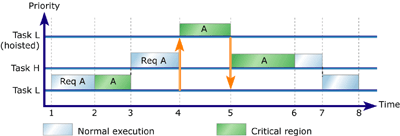
\includegraphics[scale=1]{figprot.png}\\
  \caption{An example of the priority ceiling protocol}\label{figprot}
\end{figure}
Look at figure \ref{figprot}. The explanation:
 \begin{enumerate}
   \item Task L receives control of the processor and begins executing.
\begin{enumerate}
   \item The task makes a request for Resource A.
 \end{enumerate}
\item Task L is granted ownership of Resource A and enters its critical region.
\item Task L is preempted by Task H, a higher-priority task.
      \begin{enumerate}
   \item Task H begins executing and requests ownership of Resource A, which is owned by Task L.
 \end{enumerate}
\item Task L is hoisted to a priority above Task H and resumes executing its critical region.
\item Task L releases Resource A and is lowered back to its original priority.
  \begin{enumerate}
   \item Task H acquires ownership of Resource A and begins executing its critical region.
    \end{enumerate}

\item Task H releases Resource A and continues executing normally.
\item Task H finishes executing and Task L continues executing normally.
\item Task L finishes executing.

\end{enumerate}
\end{example}

\subsection{Tasks with $D_i \leq T_i$}
We also made the assumption that the deadline $D_I$ of a task $\tau_i$ is the 
same as his period $T_i$. Dropping this assumption will lead to more 
complex formulas.  The Rate-Monotonic scheduling algorithm doesn't depend on 
this, only the schedulability tests must be reformulated. We reformulate the schedulability test 1 for RMS 
as an example.

\begin{theorem}\textbf{Schedulability test 1 for RMS - adjusted for $D_i \leq T_i$}
A feasible schedule will always exist for a task set $n $if  
 \begin{eqnarray}
  \forall j \in [1 ...n]: \sum\limits_{i=1}^j: \frac{C_i}{T_i} \leq \mathcal{U}\left(\frac{D_j}{T_j}\right)  
   \end{eqnarray}
with
 \begin{eqnarray}
    \mathcal{U}\left(\frac{D_j}{T_j}\right)  =\left\{
    \begin{array}{ll}
		2j\frac{D_j}{T_j}^{\frac{1}{j}} - j  + \frac{D_j}{T_j} + 1 & \mbox{if } \frac{1}{2}\leq \frac{D_j}{T_j} \leq 1\\
		\frac{D_j}{T_j} & \mbox{if } 0 \leq \frac{D_j}{T_j} \leq \frac{1}{2}
	\end{array}\right
  \end{eqnarray}



\end{theorem}\label{bound3}
If $D_j = T_j$, then $\frac{D_j}{T_j} = 1$, we become that $\mathcal{U}(1) = j(2^\frac{1}{j} - 
1)$, this exactly the `normal' formula we became in \ref{bound}!

The RT-test is adjusted in the same way. 

\subsection{Other extensions}
There are a lot more extensions for rate monotonic analysis to make it more widely applicable. 
By example \cite{3} explains how to deal with context switching overhead an 
preemption by fixed priority interrupt task. \cite{4} explains a protocol for a 
rate monotonic scheduling algorithm that can handle changes (addition, deletion) 
of tasks during the execution of a task set. There is also research about 
statistical rate-monotonic scheduling.
\newpage
\section{Simulations using the schedulability analysis tool Cheddar}
\subsection{What is Cheddar?}
There are a number of tools available where a developer can do a schedulability 
analysis and a calculation of response times. Initially, I planned to use 
rapidRMA from Tri-Pac software, but you need a free license key for this 
software package that you can obtain by sending them an e-mail. Unfortunately, 
after two weeks I still had no answer. I decided to use Cheddar instead. Cheddar 
is a free real time scheduling tool designed for checking task temporal 
constraints of a real time application/system. Cheddar is an open-source tool 
developed by members from the LISyC laboratory of the Universit\'{e} de Bretagne 
Occidentale and Ellidiss Technologies. It can be downloaded from
\url{http://beru.univ-brest.fr/~singhoff/cheddar/}.
\subsection{Configuration}
To configure the simulator Cheddar, I refer to the install package itself: in 
the folder \verb"/project_examples/xml" you can find very clear examples that 
are straightforward to change. The idea is that you first define a configuration 
(which processors, memory, tasks, resources,...). 
\subsection{Simulation of RMS of example \ref{goei}}
We retake example \label{goei} and will simulate it by Cheddar. We define a single processor 
and the RMS schedular. In the next figures, some screenshots are given. The 
result you can find in \ref{result}

\begin{enumerate}
    \item $\tau_1$: $T_1 = D_1$ = 4 ms,  $C_1$ = 1 ms,
    \item $\tau_2$: $T_2 = D_2$ = 5 ms,  $C_2$ = 2 ms,
    \item  $\tau_3$: $T_3 = D_3$ = 7 ms,   $C_3$ = 2 ms,
  \end{enumerate}
Just as in our calculations in the example, we become indeed that task 3 will miss it's deadline. The task set is not 
schedulable.

\begin{figure}
  \centering
  % Requires \usepackage{graphicx}
  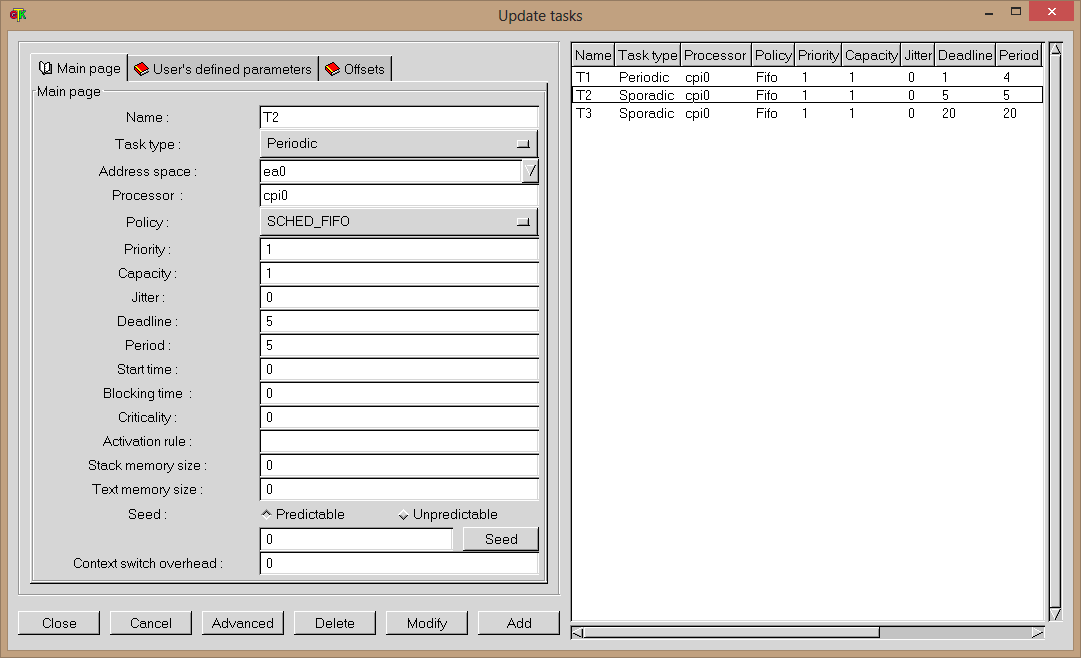
\includegraphics[scale=0.5]{task.png}\\
  \caption{Adding the tasks for the simulation.}\label{result}
\end{figure}

\begin{figure}
  \centering
  % Requires \usepackage{graphicx}
  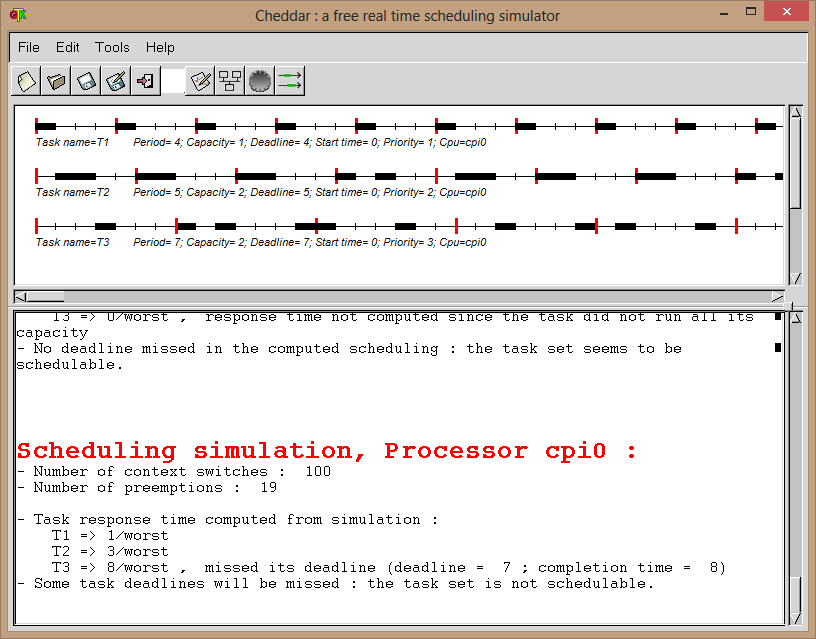
\includegraphics[scale=0.68]{result.png}\\
  \caption{The simulation with Cheddar gives the expected result.}\label{result}
\end{figure}
\newpage
\section{Conclusion}
This paper gave an overview of rate-monotonic scheduling. In the first section, we contextualize the subject in the area where RMS is used.
Next, the algorithm and al the needed terminology and definitions were
 introduced in an easy configuration with a lot of assumptions on the tasks. We 
 also introduced the schedulability tests needed to analyze wether a certain 
 task set can be scheduled with rate-monotonic scheduling or not. In the next section, 
 we dived into some extensions. In the first chapter we made a lot of 
 assumptions about the tasks being executed by RMS, but now we take a look at 
 RMS-adaptations applied on other settings, often these are much more general cases. The last chapter finally gives some concrete examples 
 of  simulations of RMS.
 \newpage
\begin{thebibliography}{99}
\bibitem{1} Fowler, Priscilla., \& Levine, Linda. (1993). \emph{Technology Transition Push: A Case Study of Rate Monotonic Analysis (Part 1)} (CMU/SEI-93-TR-029 ). Retrieved January 06, 2014, from the Software Engineering Institute, Carnegie 
Mellon University.
\bibitem{2} Jones, Michael. How to user priority inheritance, retrieved from, 
\textit{http://www.embedded.com/design/configurable-systems/4024970/How-to-use-priority-inheritance}, 
on 7, january 2013
\bibitem{3} Obenza, Ray, and Mendal, Geoff. \textit{Guaranteeing Real Time Performance Using RMA}, The Embedded Systems Conference, San Jose, CA, 1998
\bibitem{4} Sha, L., R. Rajkumar, and S. Sathaye. Priority inheritance protocols: An approach to real-time synchronization. IEEE Transactions on Computers, 39 (9), 1175-1185: 1990.
\bibitem{5} Sha, Lui, Klein, Mark H., and Goodenough, John B. \textit{Rate Monotonic Analysis}, Technical Report CMU/SEI-91-TR-6 ESD-91-TR-6, March 1991.
\bibitem{6}F. Singhoff, J. Legrand, L. Nana, L. Marcé. \textit{Cheddar : a Flexible Real Time Scheduling Framework}. ACM SIG Ada Ada Letters, volume 24, number 4, pages 1-8. Edited by ACM Press, New York, USA. December 2004, ISSN:1094-3641.   
\bibitem{6}F. Singhoff, J. Legrand, L. Nana, L. Marcé. \textit{Extending Rate Monotonic Analysis when Tasks Schare Buffers}. University of Brest. 

\bibitem{7},Nate Forman. \textit{Rate Monotonic Theory
}.
\bibitem{7}Frank Drews,. \textit{Rate Monotonic Scheduling
}.
   
   
 \end{thebibliography}
   
\end{document}

